\documentclass[9pt,twocolumn,a4paper]{extarticle}

\usepackage{amsmath}
\usepackage{fontspec}
\usepackage{unicode-math}
\setmainfont{CharisSIL-Regular.ttf}[BoldFont=CharisSIL-Bold.ttf,ItalicFont=CharisSIL-Italic.ttf,BoldItalicFont=CharisSIL-BoldItalic.ttf]
\setmathfont{STIXTwoMath-Regular.otf}
\setmonofont{consola.ttf}[BoldFont=consolab.ttf,ItalicFont=consolai.ttf,Scale=0.9]
\usepackage[top=1.5cm,bottom=2.3cm,left=1.35cm,right=1.35cm,columnsep=0.75cm,footskip=0.9cm,headsep=0.45cm]{geometry}
\usepackage{graphicx}
\usepackage{booktabs}
\usepackage{array}
\usepackage{xcolor}
\usepackage{titlesec}
\usepackage{caption}
\usepackage{float}
\usepackage{xtab}
\usepackage{listings}
\usepackage{fancyvrb}
\usepackage{tikz}
\usetikzlibrary{arrows.meta,positioning}
\tikzset{
  pbox/.style={draw=linkblue,thick,rounded corners=2pt,fill=linkblue!8,align=center,
               minimum height=9mm,text width=21mm,font=\footnotesize},
  pmine/.style={pbox,fill=linkblue!25,very thick},
  parr/.style={-{Stealth[length=2mm]},thick},
  plab/.style={font=\scriptsize,midway,fill=white,inner sep=1pt}}
\usepackage{fancyhdr}
\usepackage{setspace}
\usepackage{microtype}

\definecolor{linkblue}{RGB}{0,106,150}
\definecolor{bannergray}{RGB}{229,229,229}
\usepackage[colorlinks=true,linkcolor=linkblue,citecolor=linkblue,urlcolor=linkblue]{hyperref}

\titleformat{\section}{\normalsize\bfseries}{\thesection.}{0.55em}{}
\titleformat{\subsection}{\small\itshape}{\thesubsection.}{0.55em}{}
\titlespacing*{\section}{0pt}{10pt}{4pt}
\titlespacing*{\subsection}{0pt}{7pt}{3pt}
\setlength{\parskip}{0pt}
\setlength{\parindent}{1.1em}
\setlength{\arraycolsep}{2pt}
\setlength{\abovedisplayskip}{4pt}
\setlength{\belowdisplayskip}{4pt}
\renewcommand{\figurename}{Hình}
\renewcommand{\tablename}{Bảng}
\renewcommand{\refname}{Tài liệu tham khảo}
\captionsetup{font={footnotesize},labelfont=bf,labelsep=period,justification=justified,singlelinecheck=false,skip=3pt}
\captionsetup[table]{position=top}
\emergencystretch=3em
\setlength{\textfloatsep}{9pt plus 2pt minus 2pt}
\setlength{\floatsep}{7pt plus 2pt minus 2pt}
\setlength{\intextsep}{7pt plus 2pt minus 2pt}
\linespread{1.04}
\raggedbottom

\lstset{basicstyle=\ttfamily\fontsize{7.2}{8.4}\selectfont,breaklines=true,breakindent=1.5em,breakautoindent=true,postbreak={\mbox{\textcolor{gray}{$\hookrightarrow$}\space}},frame=single,
  rulecolor=\color{gray!55},backgroundcolor=\color{gray!5},xleftmargin=2pt,xrightmargin=2pt,
  framesep=2pt,aboveskip=1pt,belowskip=3pt,columns=fullflexible,keepspaces=true}
\renewcommand{\lstlistingname}{Mã}
\lstset{numbers=none,keywordstyle=\bfseries,commentstyle=\itshape,
  showstringspaces=false,captionpos=t,frame=tb,rulecolor=\color{black},backgroundcolor=\color{white},
  framerule=0.5pt,aboveskip=0pt,belowskip=0pt,xleftmargin=1pt,xrightmargin=1pt,framexleftmargin=3pt,
  framexrightmargin=2pt,breaklines=true,breakindent=0pt,tabsize=2}
\captionsetup[lstlisting]{skip=2pt,font={footnotesize}}

\newcommand{\code}[1]{\texttt{#1}}
\newcommand{\srcref}[1]{\par\noindent\fcolorbox{red}{white}{\footnotesize\textbf{Mã nguồn: Listing~\ref{#1} (Phụ lục~\ref{app:code}).}}\par\vspace{3pt}}
\newcommand{\spaced}[1]{\textls[160]{#1}}

\newcommand{\runauthor}{\textit{L.\,A.\ Kiet}}
\newcommand{\runtitle}{\textit{CocCoc Plus: máy tìm kiếm tiếng Việt và trình duyệt mini}}
\pagestyle{fancy}
\fancyhf{}
\renewcommand{\headrulewidth}{0pt}
\fancyhead[L]{\footnotesize\runauthor}
\fancyhead[R]{\footnotesize\runtitle}
\fancyfoot[C]{\footnotesize\thepage}
\fancypagestyle{first}{%
  \fancyhf{}\renewcommand{\headrulewidth}{0pt}%
}

\makeatletter
\renewcommand\@biblabel[1]{\textcolor{linkblue}{[#1]}}
\makeatother

\begin{document}
\thispagestyle{first}

\twocolumn[{%
\begin{@twocolumnfalse}
\vspace{-0.3cm}
\begin{center}\small\color{linkblue}Cấu trúc dữ liệu và giải thuật, Báo cáo đồ án môn học (2026)\end{center}
\vspace{-0.1cm}
\noindent\rule{\textwidth}{0.5pt}\\[-2pt]
\noindent\colorbox{bannergray}{\parbox{\dimexpr\textwidth-2\fboxsep}{\centering\vspace{3pt}
  {\small Môn học: Cấu trúc dữ liệu và giải thuật \;$\cdot$\; Trường Đại học Quốc tế, ĐHQG-HCM}\\[7pt]
  {\Large Báo cáo đồ án môn học: CocCoc Plus}\vspace{4pt}}}\\[-1pt]
\noindent\rule{\textwidth}{2.2pt}

\vspace{0.55cm}
{\fontsize{16.5}{20}\selectfont CocCoc Plus: máy tìm kiếm tiếng Việt tự cài đặt\\và trình duyệt mini\par}
\vspace{0.4cm}
{\large Lê Anh Kiệt\textsuperscript{\,a}\par}
\vspace{0.2cm}
{\scriptsize\textsuperscript{a}\,\textit{Trường Đại học Quốc tế, Đại học Quốc gia TP. Hồ Chí Minh, Việt Nam} \quad MSSV: ITCSIU24047\par}
\vspace{0.3cm}
\noindent\rule{\textwidth}{0.4pt}
\vspace{0.25cm}

\noindent\begin{minipage}[t]{0.255\textwidth}
{\footnotesize\spaced{T H Ô N G \ \ T I N}\par}
\vspace{2pt}\noindent\rule{\linewidth}{0.4pt}\par\vspace{3pt}
{\scriptsize Sinh viên: Lê Anh Kiệt\\[3pt]
\textit{Từ khóa:}\\
Máy tìm kiếm\\
Chỉ mục đảo, VByte\\
Tách từ tiếng Việt\\
BM25, PageRank\\
Trie, Bloom filter, heap\\
Web crawler\par}
\end{minipage}\hfill
\begin{minipage}[t]{0.715\textwidth}
{\footnotesize\spaced{T Ó M \ \ T Ắ T}\par}
\vspace{2pt}\noindent\rule{\linewidth}{0.4pt}\par\vspace{3pt}
{\scriptsize\setlength{\parindent}{0pt}\linespread{1.08}\selectfont
Tìm kiếm tiếng Việt khó hơn tiếng Anh ở một điểm: dấu cách ngăn các âm tiết chứ không ngăn các từ. ``Nhà hàng xóm'' có thể là ``nhà hàng'' cộng ``xóm'' hoặc ``nhà'' cộng ``hàng xóm'', và máy tìm kiếm phải chọn đúng trước khi lập chỉ mục. Trong đồ án này, em viết CocCoc Plus, một máy tìm kiếm tiếng Việt kèm trình duyệt mini để truy vấn nó.

Em tự cài đặt mọi cấu trúc dữ liệu và thuật toán lõi, không dùng thư viện tìm kiếm có sẵn như Lucene. Crawler tải trang từ 19 trang báo hạt giống. Bộ tách từ ghép âm tiết thành từ bằng quy hoạch động. Chỉ mục đảo lưu posting list đã nén bằng delta và VByte. Kết quả được chấm điểm bằng TF-IDF hoặc BM25, cộng thêm PageRank và độ khớp tiêu đề.

Sáu cấu trúc dữ liệu tự cài đứng sau các bước này: MinHeap, LRU cache, Trie, Trie theo âm tiết, Bloom filter và ma trận thưa. Phần backend gồm chín dịch vụ đứng sau một cổng vào duy nhất, còn giao diện là ứng dụng Electron.

Trên 200 truy vấn sinh tự động, BM25 đạt MRR $0{,}8989$ so với $0{,}8537$ của TF-IDF. Nén posting list giảm 75\% dung lượng so với mảng số nguyên thô.\par}
\end{minipage}

\vspace{0.25cm}
\noindent\rule{\textwidth}{0.4pt}
\vspace{0.35cm}
\end{@twocolumnfalse}
}]

%====================================================================
\section{Giới thiệu và kiến trúc}
\label{chap:intro}
%====================================================================

\subsection{Giới thiệu}
Một máy tìm kiếm làm bốn việc nối tiếp nhau \cite{manning2008ir}: tải trang về, lập chỉ mục, tìm các trang khớp truy vấn và xếp hạng chúng (Hình~\ref{fig:pipeline}). Lucene và Elasticsearch làm sẵn ba việc sau. Em không dùng chúng, vì mục tiêu của đồ án là tự viết các cấu trúc dữ liệu bên trong. Phần lõi không dùng thư viện tìm kiếm hay thư viện cấu trúc dữ liệu nào bên ngoài. Thư viện ngoài chỉ lo các việc phụ như đọc HTML (Jsoup) và đọc ghi JSON.

\begin{figure}[H]
\centering
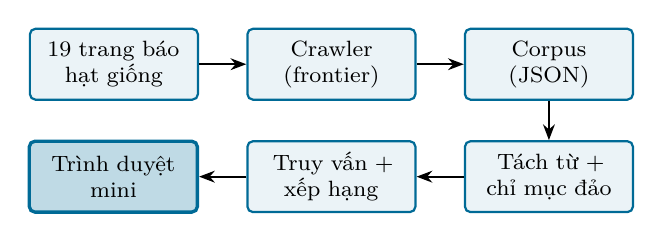
\begin{tikzpicture}[
  node distance=5mm and 6mm,
  box/.style={draw=linkblue,thick,rounded corners=2pt,fill=linkblue!8,align=center,
              minimum height=9mm,text width=19mm,font=\footnotesize},
  mine/.style={box,fill=linkblue!25,very thick},
  arr/.style={-{Stealth[length=2mm]},thick}]
  \node[box] (seed) {19 trang báo\\hạt giống};
  \node[box,right=of seed] (crawl) {Crawler\\(frontier)};
  \node[box,right=of crawl] (corpus) {Corpus\\(JSON)};
  \node[box,below=of corpus] (index) {Tách từ +\\chỉ mục đảo};
  \node[box,left=of index] (rank) {Truy vấn +\\xếp hạng};
  \node[mine,left=of rank] (app) {Trình duyệt\\mini};
  \draw[arr] (seed) -- (crawl);
  \draw[arr] (crawl) -- (corpus);
  \draw[arr] (corpus) -- (index);
  \draw[arr] (index) -- (rank);
  \draw[arr] (rank) -- (app);
\end{tikzpicture}
\caption{Đường đi của dữ liệu từ trang web đến kết quả tìm kiếm.}
\label{fig:pipeline}
\end{figure}

Báo cáo đi theo đúng đường đi này. Mỗi mục trình bày một chặng cùng cấu trúc dữ liệu mà chặng đó dùng (Bảng~\ref{tab:map}).

\begin{table}[H]
\centering
\caption{Các chặng xử lý và cấu trúc dữ liệu tương ứng.}
\label{tab:map}
\footnotesize
\begin{tabular}{@{}lp{4.6cm}l@{}}
\toprule
Chặng & Nội dung chính & Mục \\
\midrule
P1 & frontier hai tầng, MinHeap, Bloom filter & \ref{chap:p1} \\
P2 & Trie âm tiết, quy hoạch động tách từ & \ref{chap:p2} \\
P3 & chỉ mục đảo, delta + VByte & \ref{chap:p3} \\
P4 & cây truy vấn, giao posting list & \ref{chap:p4} \\
P5 & TF-IDF, BM25, PageRank, top-$K$, LRU & \ref{chap:p5} \\
P6 & Trie gợi ý, dịch vụ, trình duyệt & \ref{chap:p6} \\
\bottomrule
\end{tabular}
\end{table}

\subsection{Cấu trúc chương trình}
Thuật toán nằm trong ba thư viện ở \code{backend/java/libs}. \code{core-common} chứa các cấu trúc dữ liệu, \code{core-crawler} chứa crawler và \code{core-search} chứa chỉ mục, truy vấn và xếp hạng. Các dịch vụ chỉ là lớp vỏ HTTP mỏng bọc quanh ba thư viện này: \code{crawler-service} có 393 dòng, còn thư viện crawler bên dưới có 8.491 dòng. Hình~\ref{fig:tree} liệt kê các thư mục chính.

\begin{figure}[H]
\centering
\begin{Verbatim}[fontsize=\fontsize{5.6}{6.6}\selectfont,frame=single]
CocCoc-Plus/
|-- docker-compose.yml       # 9 dịch vụ + Postgres, Redis, Mongo
|-- run-backend.bat          # chạy backend, run-crawl.bat: crawl
|-- backend/
|   |-- java/libs/
|   |   |-- core-common/     # cấu trúc dữ liệu tự cài
|   |   |   `-- datastructure/  # MinHeap, LRUCache, Trie,
|   |   |                       # SyllableTrie, BloomFilter, SparseMatrix
|   |   |-- core-crawler/    # tải trang, lọc URL
|   |   |   |-- frontier/    # FrontQueues, BackQueues, UrlFrontier
|   |   |   `-- bus/         # sự kiện crawl (bộ nhớ hoặc Kafka)
|   |   |-- core-search/
|   |   |   |-- index/       # InvertedIndex, VByteCodec, tách từ
|   |   |   |-- query/       # QueryParser, PostingListMerger, ast/
|   |   |   |-- ranking/     # TfIdf, BM25, PageRank, decorator/
|   |   |   `-- eval/        # đo chất lượng tìm kiếm
|   |   `-- platform/        # bảo mật, giới hạn tốc độ dùng chung
|   |-- java/services/       # api-gateway, auth, search,
|   |                        # crawler, analytics
|   `-- go/services/         # history, downloads, settings, football
|-- desktop-app/             # trình duyệt mini (Electron + React)
|   `-- src/renderer/src/lib/  # Stack.ts, BookmarkTrie.ts
|-- deploy/                  # Prometheus, Grafana, init Postgres
`-- docs/                    # tài liệu từng pipeline
\end{Verbatim}
\caption{Cây thư mục của dự án (chỉ các phần chính).}
\label{fig:tree}
\end{figure}

\subsection{Chín dịch vụ}
Backend chia thành chín dịch vụ (Bảng~\ref{tab:services}). Trình duyệt chỉ nói chuyện với \code{api-gateway} ở cổng 8080. Tám dịch vụ còn lại chỉ nghe trong mạng nội bộ của Docker Compose.

\begin{table}[H]
\centering
\caption{Các dịch vụ của backend.}
\label{tab:services}
\footnotesize
\begin{tabular}{@{}p{2.3cm}rlp{3.0cm}@{}}
\toprule
Dịch vụ & Cổng & Ngôn ngữ & Phụ trách \\
\midrule
\code{api-gateway} & 8080 & Java & định tuyến, kiểm JWT \\
\code{auth-service} & 8081 & Java & tài khoản, phát JWT \\
\code{search-service} & 8082 & Java & chỉ mục, truy vấn, gợi ý \\
\code{crawler-service} & 8083 & Java & phiên crawl, lập lại chỉ mục \\
\code{analytics-service} & 8084 & Java & thống kê sử dụng \\
\code{history-service} & 8085 & Go & lịch sử duyệt (MongoDB) \\
\code{downloads-service} & 8086 & Go & danh sách tải về \\
\code{settings-service} & 8087 & Go & cài đặt người dùng \\
\code{football-service} & 8090 & Go & dữ liệu bóng đá \\
\bottomrule
\end{tabular}
\end{table}

\subsection{Dữ liệu đầu vào}
\label{sec:input}
Đầu vào của tầng chỉ mục là corpus do crawler ghi ra, tức file \code{crawled-documents.json}. Mỗi phần tử là một \code{WebDocument} (Bảng~\ref{tab:doc}). Corpus lớn nhất em đã crawl có 39.780 tài liệu và nặng $464{,}2$~MB.

\begin{table}[H]
\centering
\caption{Các trường chính của một \code{WebDocument}.}
\label{tab:doc}
\footnotesize
\begin{tabular}{@{}p{2.3cm}p{5.3cm}@{}}
\toprule
Trường & Ý nghĩa \\
\midrule
\code{docId} & số nguyên định danh, tăng dần theo thứ tự tải \\
\code{url}, \code{title} & địa chỉ đã chuẩn hóa và tiêu đề trang \\
\code{metaDescription} & mô tả lấy từ thẻ meta \\
\code{bodyText} & thân bài đã bỏ thẻ HTML \\
\code{language} & \code{vi}, \code{en} hoặc \code{und} \\
\code{outlinks} & các liên kết ra, dùng cho PageRank \\
\bottomrule
\end{tabular}
\end{table}

Crawler ghi file qua một tệp tạm rồi đổi tên. Nếu máy tắt giữa chừng, file cũ vẫn còn nguyên. Không dùng \code{--fresh} thì lần crawl sau nối tiếp corpus cũ và không tải lại các trang đã có.

%====================================================================
\section{P1: Thu thập trang web}
\label{chap:p1}
%====================================================================
Crawler chạy 32 luồng. Mỗi luồng lặp lại một việc: lấy một URL từ frontier, tải trang, rồi đưa các liên kết mới tìm được trở lại frontier. Mục này có ba phần.
\begin{itemize}\itemsep0pt
\item Phần 1, frontier hai tầng: quyết định URL nào được tải tiếp theo.
\item Phần 2, chống trùng bằng Bloom filter: nhớ các URL đã gặp.
\item Phần 3, bảy tầng lọc: loại URL và trang không cần.
\end{itemize}

\subsection{Phần 1: Frontier hai tầng}
\label{sec:frontier}
Frontier phải thỏa hai yêu cầu kéo về hai phía. Trang quan trọng nên được tải trước. Nhưng crawler cũng không được dồn nhiều request vào một máy chủ. Một hàng đợi duy nhất chỉ sắp được theo một tiêu chí. Em dùng kiến trúc hai tầng của Mercator \cite{heydon1999mercator}: tầng trước giữ độ ưu tiên, tầng sau giữ phép lịch sự (Hình~\ref{fig:frontier}).

\begin{figure}[H]
\centering
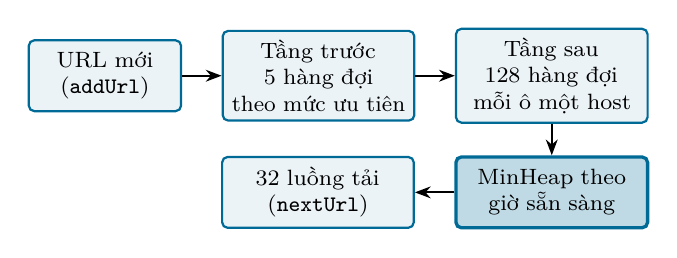
\begin{tikzpicture}[node distance=4mm and 5mm,font=\footnotesize]
\node[pbox,text width=17mm] (in) {URL mới\\(\code{addUrl})};
\node[pbox,right=of in,text width=22mm] (front) {Tầng trước\\5 hàng đợi\\theo mức ưu tiên};
\node[pbox,right=of front,text width=22mm] (back) {Tầng sau\\128 hàng đợi\\mỗi ô một host};
\node[pmine,below=of back,text width=22mm] (heap) {MinHeap theo\\giờ sẵn sàng};
\node[pbox,left=of heap,text width=22mm] (out) {32 luồng tải\\(\code{nextUrl})};
\draw[parr] (in)--(front);
\draw[parr] (front)--(back);
\draw[parr] (back)--(heap);
\draw[parr] (heap)--(out);
\end{tikzpicture}
\caption{Frontier hai tầng. Tầng trước chọn URL theo độ ưu tiên, tầng sau bảo đảm mỗi host chỉ nhận một request mỗi giây.}
\label{fig:frontier}
\end{figure}

\textbf{Mức ưu tiên.} Mỗi URL nhận một mức từ 0 đến 4, với 0 là cao nhất. Mức khởi đầu bằng độ sâu $d$ của URL tính từ hạt giống. Host có đuôi \code{.vn} được nâng một bậc, và URL có từ 5 liên kết trỏ tới trở lên cũng vậy:
\begin{equation}
\ell=\operatorname{clip}\big(d-[\text{host}\in\code{.vn}]-[\text{backlink}\ge5],\ 0,\ 4\big).
\label{eq:level}
\end{equation}

\textbf{Chọn hàng đợi tầng trước.} Nếu luôn lấy mức thấp nhất còn hàng thì các trang sâu không bao giờ tới lượt. Em chọn ngẫu nhiên có trọng số: mức $i$ trong $L$ mức có trọng số
\begin{equation}
w_i=2^{\,L-1-i},
\label{eq:weight}
\end{equation}
nên với $L=5$ mức 0 được chọn nhiều gấp 16 lần mức 4. Chỉ các hàng đợi còn hàng mới góp trọng số. Bộ sinh số ngẫu nhiên dùng hạt cố định, nên hai lần crawl cho cùng thứ tự chọn.

\srcref{lst:selector}

\textbf{Phép lịch sự ở tầng sau.} Mỗi ô trong 128 ô của tầng sau gắn với một host và có thời điểm sẵn sàng \code{availableAt}. Sau khi lấy một URL, ô đó phải chờ 1000~ms. Mỗi lần lấy, frontier cần biết ô nào tới giờ sớm nhất, và MinHeap trả lời câu hỏi này trong $O(\log n)$. Nếu phần tử nhỏ nhất của heap chưa tới giờ thì không ô nào tới giờ, và luồng ngủ tối đa 50~ms ở ngoài khối khóa.

Khóa của một phần tử đang nằm trong heap không được đổi, vì đổi sẽ phá tính chất heap. Vì vậy \code{poll} rút ô ra khỏi heap, cập nhật \code{availableAt}, rồi mới chèn lại.

\srcref{lst:backpoll}

\subsection{Phần 2: Chống trùng bằng Bloom filter}
\label{sec:bloom}
Crawler gặp cùng một URL rất nhiều lần, vì các trang báo liên kết chéo nhau dày đặc. Giữ mọi URL đã gặp trong một \code{HashSet} tốn hàng trăm MB khi crawl lớn. Bloom filter \cite{bloom1970} trả lời câu hỏi ``đã gặp chưa'' bằng một mảng bit. Câu trả lời ``chưa'' luôn đúng, còn câu trả lời ``rồi'' có thể sai với xác suất $p$.

Với $n$ phần tử dự kiến và tỉ lệ dương tính giả $p$, số bit $m$ và số hàm băm $k$ tối ưu là
\begin{equation}
m=\Big\lceil-\frac{n\ln p}{(\ln 2)^2}\Big\rceil,\qquad k=\operatorname{round}\Big(\frac{m}{n}\ln 2\Big).
\label{eq:bloom}
\end{equation}
Với $n$ bằng 200.000 và $p=1\%$, công thức cho $m$ bằng 1.917.012 bit (khoảng 234~KB) và $k=7$. Một dương tính giả làm crawler bỏ sót một trang chưa thăm. Em chấp nhận mức 1\% này để đổi lấy bộ nhớ.

Bảy chỉ số bit không cần bảy hàm băm riêng. Chương trình tính hai giá trị băm $h_1$ (FNV-1a trên các byte UTF-8) và $h_2$, rồi ghép chúng lại:
\begin{equation}
g_i(x)=\big(h_1(x)+i\,h_2(x)\big)\bmod m,\qquad i=0,\dots,k-1.
\label{eq:dhash}
\end{equation}

\srcref{lst:bloom}

\subsection{Phần 3: Bảy tầng lọc}
Mỗi URL đi qua bảy tầng chặn, xếp theo nguyên tắc tầng rẻ và loại nhiều đứng trước (Bảng~\ref{tab:filters}). Hai tầng đầu chỉ xử lý chuỗi và không chạm mạng.

\begin{table}[H]
\centering
\caption{Bảy tầng lọc của crawler, theo thứ tự chạy.}
\label{tab:filters}
\footnotesize
\begin{tabular}{@{}rp{2.3cm}p{4.6cm}@{}}
\toprule
\# & Lớp & Loại bỏ \\
\midrule
1 & \code{UrlFilter} & quá sâu, sai scheme, ngoài tên miền, file \code{.pdf}/\code{.zip}/ảnh \\
2 & \code{UrlSeenFilter} & URL đã gặp (Bloom filter) \\
3 & \code{RobotsTxtParser} & URL bị \code{robots.txt} cấm \\
4 & \code{SeedUrlValidator} & địa chỉ nội bộ (chống SSRF) \\
5 & \code{HtmlDownloader} & trang lỗi, quá 5 lần chuyển hướng \\
6 & \code{LanguageFilter} & trang không phải tiếng Việt hay tiếng Anh \\
7 & \code{ContentSeenFilter} & nội dung trùng (SHA-256 của thân bài) \\
\bottomrule
\end{tabular}
\end{table}

Tầng 2 và tầng 7 chống hai loại trùng khác nhau. Tầng 2 so URL. Tầng 7 so nội dung, vì bản in, bản AMP và bản có tham số theo dõi là cùng một bài dưới các URL khác nhau.

Tầng 4 tồn tại vì quản trị viên có thể yêu cầu crawl một URL bất kỳ. Nếu không chặn, một request tới \code{169.254.169.254} trên máy ảo đám mây sẽ trả về khóa truy cập tạm thời, và nội dung đó lọt vào chỉ mục công khai. Crawler kiểm tra địa chỉ IP sau khi phân giải DNS, trước mỗi lần tải và ở từng chặng chuyển hướng.

%====================================================================
\section{P2: Tách từ tiếng Việt}
\label{chap:p2}
%====================================================================
Chỉ mục lưu \emph{từ}, còn văn bản tiếng Việt chỉ cho sẵn \emph{âm tiết}. Bộ tách từ phải ghép các âm tiết liền nhau thành từ, ví dụ ``máy tính'' thành \code{máy\_tính}. Mục này có ba phần.
\begin{itemize}\itemsep0pt
\item Phần 1, từ điển có trọng số: mỗi từ có một điểm số.
\item Phần 2, Trie theo âm tiết: tra từ điển theo từng âm tiết.
\item Phần 3, quy hoạch động: chọn cách tách có tổng điểm lớn nhất.
\end{itemize}

\subsection{Phần 1: Từ điển có trọng số}
\label{sec:dict}
Từ điển được sinh từ dữ liệu của \code{coccoc-tokenizer} \cite{coccoctokenizer}. Mỗi từ có tần suất $f$ và số âm tiết $L$. Trọng số của từ là
\begin{equation}
w(f,L)=\big(\log_2(f+3)\big)^{a_L}\cdot L^{\,b_L},
\label{eq:wordweight}
\end{equation}
với cặp tham số $(a_L,b_L)$ riêng cho từng độ dài (Bảng~\ref{tab:param}). Tần suất trải từ 10 đến hơn 2 tỉ, nên công thức lấy logarit để một từ rất phổ biến không lấn át mọi từ khác. Số 3 được cộng vào để từ có $f=1$ vẫn có trọng số khác 0.

\begin{table}[H]
\centering
\caption{Tham số của công thức \eqref{eq:wordweight}, lấy từ \code{coccoc-tokenizer}.}
\label{tab:param}
\footnotesize
\begin{tabular}{@{}lrrrr@{}}
\toprule
Số âm tiết $L$ & 1 & 2 & 3 & 4 \\
\midrule
$a_L$ (mũ của tần suất) & $0{,}38$ & $0{,}14$ & $1{,}42$ & $1{,}45$ \\
$b_L$ (mũ của độ dài) & $1{,}00$ & $2{,}59$ & $4{,}42$ & $0{,}23$ \\
\bottomrule
\end{tabular}
\end{table}

Bảng tham số chỉ có bốn cột, nên từ dài nhất mà bộ tách từ nhận là bốn âm tiết.

\subsection{Phần 2: Trie theo âm tiết}
\label{sec:strie}
Trie thông thường đi theo từng ký tự. \code{SyllableTrie} đi theo từng âm tiết: mỗi cạnh là một âm tiết, và nút kết thúc một từ thì lưu trọng số của từ đó (Hình~\ref{fig:strie}).

\begin{figure}[H]
\centering
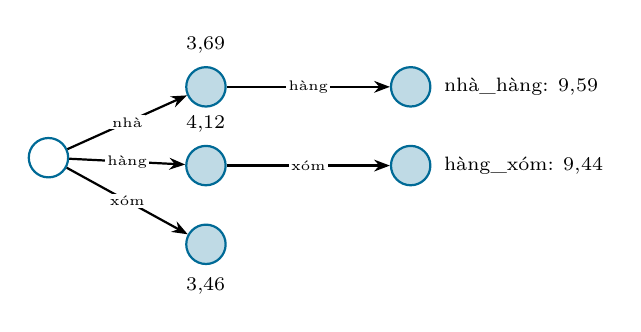
\begin{tikzpicture}[font=\scriptsize,
  nd/.style={circle,draw=linkblue,thick,inner sep=1.2pt,minimum size=5mm},
  wd/.style={nd,fill=linkblue!25},
  lv/.style={font=\tiny,midway,fill=white,inner sep=0.8pt}]
\node[nd] (r) at (0,0) {};
\node[wd] (nha) at (2.0,0.9) {};
\node[wd] (hang) at (2.0,-0.1) {};
\node[wd] (xom) at (2.0,-1.1) {};
\node[wd] (nhahang) at (4.6,0.9) {};
\node[wd] (hangxom) at (4.6,-0.1) {};
\draw[parr] (r)--node[lv]{nhà} (nha);
\draw[parr] (r)--node[lv]{hàng} (hang);
\draw[parr] (r)--node[lv]{xóm} (xom);
\draw[parr] (nha)--node[lv]{hàng} (nhahang);
\draw[parr] (hang)--node[lv]{xóm} (hangxom);
\node[above=1pt] at (nha.north) {$3{,}69$};
\node[above=1pt] at (hang.north) {$4{,}12$};
\node[below=1pt] at (xom.south) {$3{,}46$};
\node[right=1pt] at (nhahang.east) {nhà\_hàng: $9{,}59$};
\node[right=1pt] at (hangxom.east) {hàng\_xóm: $9{,}44$};
\end{tikzpicture}
\caption{Một phần của Trie âm tiết. Nút tô đậm kết thúc một từ và mang trọng số của từ đó.}
\label{fig:strie}
\end{figure}

Trie không tạo một đối tượng cho mỗi nút. Mỗi âm tiết được đổi thành một số nguyên bắt đầu từ 1. Các cạnh nằm trong một bảng băm địa chỉ mở, với khóa là một số \code{long} gói cả nút cha và mã âm tiết: $(\text{cha}\ll32)\mid\text{mã}$. Khi đụng độ, chương trình dò tuyến tính sang ô kế. Bảng tăng gấp đôi khi đầy quá 55\%.

Cách lưu này có hai lợi ích so với \code{HashMap<String, Double>}. Nó tránh hàng trăm nghìn đối tượng nút. Và khi một nút không có cạnh cho âm tiết kế tiếp, bộ tách từ biết ngay rằng không từ nào trong từ điển bắt đầu bằng dãy âm tiết đó, nên dừng tìm sớm. Một \code{HashMap} chỉ trả lời được ``chuỗi này có phải là từ không'', nên phải thử lần lượt cả bốn độ dài.

\subsection{Phần 3: Quy hoạch động}
\label{sec:dp}
Cách tách đơn giản nhất là tham lam: tại mỗi vị trí, lấy từ dài nhất có trong từ điển. Với ``nhà hàng xóm'', cách này lấy ngay ``nhà hàng'' và để lại ``xóm''. Kết quả sai, và thuật toán không quay lại sửa được vì nó đã dùng mất âm tiết ``hàng''.

Em tìm cách tách có tổng trọng số lớn nhất trên cả câu. Gọi $\text{best}[j]$ là tổng trọng số lớn nhất khi tách $j$ âm tiết đầu:
\begin{equation}
\text{best}[0]=0,\qquad
\text{best}[j]=\max_{\,j-4\le i<j}\Big(\text{best}[i]+w\big(s_i\dots s_{j-1}\big)\Big).
\label{eq:dp}
\end{equation}
Đây là bài toán đường đi dài nhất trên một đồ thị có hướng không chu trình. Đỉnh là ranh giới giữa các âm tiết, còn cạnh $i\to j$ là một từ trong từ điển (Hình~\ref{fig:dag}). Mọi cạnh đi từ chỉ số nhỏ đến chỉ số lớn, nên một lượt quét từ trái sang phải là đủ. Mỗi đỉnh có tối đa bốn cạnh ra, do đó độ phức tạp là $O(n)$ với $n$ âm tiết.

\begin{figure}[H]
\centering
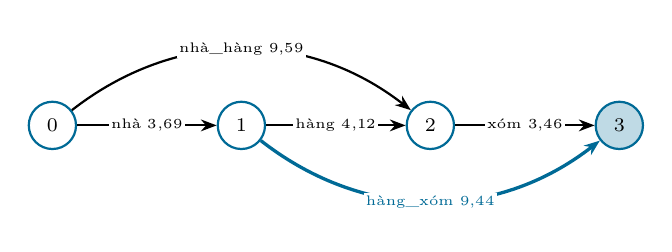
\begin{tikzpicture}[font=\scriptsize,
  nd/.style={circle,draw=linkblue,thick,inner sep=1pt,minimum size=6mm},
  lv/.style={font=\tiny,midway,fill=white,inner sep=0.8pt}]
\node[nd] (n0) at (0,0) {0};
\node[nd] (n1) at (2.4,0) {1};
\node[nd] (n2) at (4.8,0) {2};
\node[nd,fill=linkblue!25] (n3) at (7.2,0) {3};
\draw[parr] (n0)--node[lv]{nhà $3{,}69$} (n1);
\draw[parr] (n1)--node[lv]{hàng $4{,}12$} (n2);
\draw[parr] (n2)--node[lv]{xóm $3{,}46$} (n3);
\draw[parr] (n0) to[bend left=38] node[lv]{nhà\_hàng $9{,}59$} (n2);
\draw[parr,very thick,linkblue] (n1) to[bend right=38] node[lv]{hàng\_xóm $9{,}44$} (n3);
\end{tikzpicture}
\caption{Đồ thị tách từ của ``nhà hàng xóm''. Đường tốt nhất là $0\to1\to3$ với tổng $3{,}69+9{,}44=13{,}13$, lớn hơn $9{,}59+3{,}46=13{,}05$ của cách tách tham lam.}
\label{fig:dag}
\end{figure}

Bảng~\ref{tab:dptrace} ghi lại giá trị của hai mảng sau khi chạy. Mảng \code{trace} lưu đỉnh đứng trước trên đường tốt nhất. Truy ngược từ đỉnh 3 cho các ranh giới $[0,1,3]$, tức hai từ \code{nhà} và \code{hàng\_xóm}.

\begin{table}[H]
\centering
\caption{Hai mảng quy hoạch động cho ``nhà hàng xóm''.}
\label{tab:dptrace}
\footnotesize
\begin{tabular}{@{}lrrrr@{}}
\toprule
$j$ & 0 & 1 & 2 & 3 \\
\midrule
\code{best[j]} & 0 & $3{,}69$ & $9{,}59$ & $13{,}13$ \\
\code{trace[j]} & & 0 & 0 & 1 \\
\bottomrule
\end{tabular}
\end{table}

Tên riêng và từ mượn không có trong từ điển. Để đồ thị luôn có đường từ 0 đến $n$, mỗi đỉnh có thêm một cạnh sang đỉnh kế với trọng số $0{,}5$, ứng với việc tách riêng một âm tiết lạ. Trọng số này thấp hơn mọi từ trong từ điển, nên cạnh này chỉ được dùng khi không còn cách nào khác.

\srcref{lst:segment}

%====================================================================
\section{P3: Chỉ mục đảo và nén}
\label{chap:p3}
%====================================================================
Chỉ mục đảo trả lời câu hỏi ``từ này xuất hiện trong những tài liệu nào'' mà không phải đọc lại corpus. Mục này có ba phần.
\begin{itemize}\itemsep0pt
\item Phần 1, cấu trúc chỉ mục: từ điển term và posting list.
\item Phần 2, nén posting list: delta và VByte.
\item Phần 3, bộ nhớ: ba tối ưu và số đo.
\end{itemize}

\subsection{Phần 1: Cấu trúc chỉ mục}
\label{sec:index}
Chỉ mục là một ánh xạ từ term sang posting list (Hình~\ref{fig:inverted}). Mỗi posting gồm \code{docId} của một tài liệu chứa term và các vị trí của term trong tài liệu đó. Số vị trí chính là tần suất $tf$, nên chỉ mục không lưu $tf$ riêng.

\begin{figure}[H]
\centering
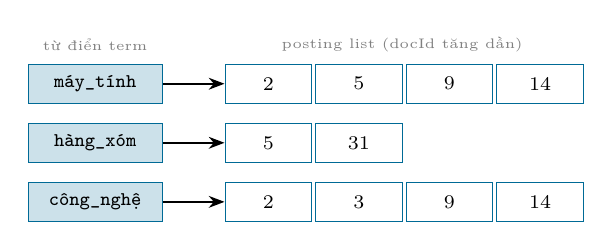
\begin{tikzpicture}[font=\scriptsize,
  cell/.style={draw=linkblue,minimum height=5mm,minimum width=11mm,inner sep=1pt},
  term/.style={cell,fill=linkblue!20,minimum width=17mm}]
\node[term] (t1) at (0,0) {\code{máy\_tính}};
\node[term] (t2) at (0,-0.75) {\code{hàng\_xóm}};
\node[term] (t3) at (0,-1.5) {\code{công\_nghệ}};
\foreach \i/\d in {0/2,1/5,2/9,3/14}
  \node[cell] (a\i) at (2.2+\i*1.15,0) {\d};
\foreach \i/\d in {0/5,1/31}
  \node[cell] (b\i) at (2.2+\i*1.15,-0.75) {\d};
\foreach \i/\d in {0/2,1/3,2/9,3/14}
  \node[cell] (c\i) at (2.2+\i*1.15,-1.5) {\d};
\draw[parr] (t1)--(a0); \draw[parr] (t2)--(b0); \draw[parr] (t3)--(c0);
\node[font=\tiny,gray] at (0,0.5) {từ điển term};
\node[font=\tiny,gray] at (3.9,0.5) {posting list (docId tăng dần)};
\end{tikzpicture}
\caption{Chỉ mục đảo. Mỗi term trỏ tới danh sách \code{docId} đã sắp tăng dần.}
\label{fig:inverted}
\end{figure}

Tài liệu được thêm vào theo thứ tự \code{docId} tăng dần, nên mọi posting list luôn sắp sẵn. Tính chất này được kiểm tra khi thêm tài liệu, và ba việc phía sau dựa vào nó: nén delta, tìm nhị phân một tài liệu trong posting list, và giao hai danh sách trong thời gian tuyến tính.

Khi lập chỉ mục, tiêu đề, mô tả và thân bài của tài liệu được nối lại rồi tách từ. Bộ tách từ của truy vấn và của chỉ mục là cùng một lớp, vì nếu hai bên tách khác nhau thì term của truy vấn sẽ không khớp term trong chỉ mục.

\subsection{Phần 2: Nén posting list}
\label{sec:vbyte}
Một \code{docId} kiểu \code{int} tốn 4 byte dù giá trị nhỏ hay lớn. Việc nén gồm hai bước.

\textbf{Delta.} Vì danh sách tăng dần, chương trình lưu hiệu giữa hai phần tử liền nhau thay cho giá trị gốc. Dãy $1002,\,1005,\,1009$ trở thành $1002,\,3,\,4$. Term càng phổ biến thì các hiệu càng nhỏ.

\textbf{VByte.} Mỗi số được ghi bằng số byte vừa đủ \cite{manning2008ir}. Mỗi byte mang 7 bit dữ liệu. Bit cao nhất bằng 1 nếu còn byte tiếp theo và bằng 0 ở byte cuối. Số nhỏ hơn 128 chỉ tốn 1 byte. Ví dụ với số 300:
\begin{equation}
300=\underbrace{10}_{\text{cao}}\,\underbrace{0101100}_{\text{thấp}}{}_2
\;\longrightarrow\;
\underbrace{1\,0101100}_{\code{0xAC}}\ \ \underbrace{0\,0000010}_{\code{0x02}},
\label{eq:vbyte}
\end{equation}
tức 2 byte thay vì 4.

\srcref{lst:vbyte}

Mỗi term có một khối byte riêng. Một truy vấn chỉ chạm vài term trong hàng trăm nghìn term, nên chương trình chỉ giải nén đúng các khối cần đọc. Nén cả file bằng GZIP cho tỉ lệ tốt hơn vài điểm phần trăm, nhưng muốn đọc một term thì phải giải nén toàn bộ. Thân bài thì khác: nó luôn được đọc trọn một tài liệu để sinh đoạn trích, nên em nén nó bằng Deflate.

\subsection{Phần 3: Bộ nhớ}
Bảng~\ref{tab:compress} so dung lượng posting list trước và sau khi nén, đo trên corpus 5.011 tài liệu có 1.594.938 posting và 3.821.061 vị trí.

\begin{table}[H]
\centering
\caption{Dung lượng posting list trên corpus 5.011 tài liệu.}
\label{tab:compress}
\footnotesize
\begin{tabular}{@{}lrr@{}}
\toprule
Thành phần & Thô (MB) & Đã nén (MB) \\
\midrule
\code{docId} & $6{,}4$ & $1{,}6$ \\
$tf$ & $6{,}4$ & 0 (bỏ hẳn) \\
Chỉ số bắt đầu của vị trí & & $1{,}6$ \\
Vị trí & $15{,}3$ & $3{,}8$ \\
\midrule
Tổng & $28{,}1$ & $7{,}0$ \\
\bottomrule
\end{tabular}
\end{table}

Dung lượng còn 25\% so với mảng số nguyên thô. Phần tiết kiệm lớn hơn nữa đến từ việc bỏ đối tượng: $1{,}59$ triệu đối tượng \code{Posting} và $1{,}59$ triệu mảng vị trí tốn khoảng 76~MB chỉ riêng phần header, còn ba mảng byte phẳng thì không có header cho từng phần tử.

Hai tối ưu khác cũng nhắm vào số đối tượng. \code{TermDictionary} giữ một bản duy nhất cho mỗi chuỗi term (mẫu Flyweight \cite{gamma1994design}), vì cùng một term xuất hiện hàng triệu lần trong lúc lập chỉ mục. Vị trí được lưu bằng \code{int[]} thay cho \code{List<Integer>}. Trên corpus 2.518 trang, chỉ mục chiếm khoảng 123~MB bộ nhớ. Nếu bỏ \code{TermDictionary}, quay về \code{List<Integer>} và không nén thân bài thì con số này tăng thêm khoảng 464~MB.

%====================================================================
\section{P4: Xử lý truy vấn}
\label{chap:p4}
%====================================================================
Chặng này biến chuỗi người dùng gõ thành tập tài liệu ứng viên. Mục này có ba phần.
\begin{itemize}\itemsep0pt
\item Phần 1, phân tích cú pháp: chuỗi truy vấn thành cây.
\item Phần 2, giao posting list: tìm tài liệu chứa mọi term.
\item Phần 3, cụm từ và trường hợp không có kết quả.
\end{itemize}

\subsection{Phần 1: Phân tích cú pháp}
\label{sec:parser}
\code{QueryParser} hiểu bốn loại cú pháp (Bảng~\ref{tab:syntax}). Kết quả là một cây, trong đó mỗi nút biết tự tính tập tài liệu của mình (Hình~\ref{fig:ast}).

\begin{table}[H]
\centering
\caption{Cú pháp truy vấn.}
\label{tab:syntax}
\footnotesize
\begin{tabular}{@{}p{2.6cm}p{5.0cm}@{}}
\toprule
Cú pháp & Ý nghĩa \\
\midrule
\code{a b} & chứa cả hai từ (AND, mặc định) \\
\code{"a b"} & chứa đúng cụm từ, các từ đứng liền nhau \\
\code{a OR b} & chứa ít nhất một trong hai từ \\
\code{-a} & không chứa từ này \\
\code{site:vnexpress.net} & chỉ lấy tài liệu của host này \\
\bottomrule
\end{tabular}
\end{table}

\begin{figure}[H]
\centering
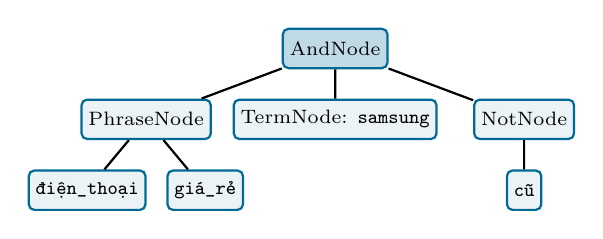
\begin{tikzpicture}[font=\scriptsize,
  nd/.style={draw=linkblue,thick,rounded corners=2pt,fill=linkblue!8,inner sep=2.5pt,minimum height=5mm},
  level distance=9mm,sibling distance=24mm,
  edge from parent/.style={draw,thick}]
\node[nd,fill=linkblue!25] {AndNode}
  child {node[nd] {PhraseNode}
    child[sibling distance=15mm] {node[nd] {\code{điện\_thoại}}}
    child[sibling distance=15mm] {node[nd] {\code{giá\_rẻ}}}}
  child {node[nd] {TermNode: \code{samsung}}}
  child {node[nd] {NotNode}
    child {node[nd] {\code{cũ}}}};
\end{tikzpicture}
\caption{Cây của truy vấn \code{"điện thoại giá rẻ" samsung -cũ}.}
\label{fig:ast}
\end{figure}

Nút loại trừ không đứng một mình được, vì phần bù của một posting list là gần như cả corpus. \code{AndNode} tính giao của các nút con còn lại trước, rồi mới trừ đi tập của \code{NotNode}. Phép trừ hai danh sách đã sắp dùng hai con trỏ và tốn $O(m+n)$.

\subsection{Phần 2: Giao posting list}
\label{sec:merge}
Giao hai danh sách đã sắp là thao tác chạy nhiều nhất của chặng này. Thuật toán hai con trỏ cơ bản tốn $O(m+n)$: so hai phần tử đầu, bằng nhau thì ghi nhận, nếu không thì tiến con trỏ đang trỏ vào số nhỏ hơn.

Khi một danh sách ngắn và một danh sách dài, phần lớn các bước tiến trên danh sách dài là lãng phí. \code{PostingCursor} có thêm thao tác \code{skipTo(t)}, nhảy thẳng tới phần tử đầu tiên có $\text{docId}\ge t$. Thao tác này gồm hai pha. Pha một nhảy các bước $1,2,4,8,\dots$ cho tới khi vượt qua $t$. Pha hai tìm nhị phân trong đoạn vừa khoanh được. Chi phí là $O(\log d)$, với $d$ là khoảng cách thật sự phải nhảy, và không phụ thuộc độ dài cả danh sách.

\srcref{lst:skipto}

\srcref{lst:intersect}

Khi truy vấn có nhiều term, các posting list được sắp theo độ dài và giao từ ngắn đến dài. Kết quả trung gian không bao giờ dài hơn danh sách ngắn nhất, nên mỗi bước sau làm việc trên một tập nhỏ. Nếu kết quả trung gian đã rỗng thì vòng lặp dừng ngay.

\subsection{Phần 3: Cụm từ và trường hợp không có kết quả}
Với truy vấn cụm từ, chương trình trước hết giao posting list của các term trong cụm. Sau đó, với từng tài liệu ứng viên, nó kiểm tra bằng mảng vị trí: phải có một vị trí $p$ của term đầu sao cho term thứ $i$ nằm ở vị trí $p+i$. Mảng vị trí đã sắp tăng dần, nên mỗi lần kiểm tra là một phép tìm nhị phân.

Một truy vấn dài như ``máy tính xách tay giá rẻ cho sinh viên'' hiếm khi có tài liệu chứa đủ mọi term. Khi phép AND cho tập rỗng, \code{CandidateResolver} lùi dần về phép AND trên các tập con của term thay vì trả về danh sách trống. Tập ứng viên cuối cùng được cắt ở một trần để chặng xếp hạng không phải chấm điểm cả corpus.

%====================================================================
\section{P5: Xếp hạng}
\label{chap:p5}
%====================================================================
Chặng cuối chấm điểm từng ứng viên và giữ lại các tài liệu điểm cao nhất. Mục này có năm phần.
\begin{itemize}\itemsep0pt
\item Phần 1, TF-IDF: mô hình không gian vector.
\item Phần 2, BM25: mô hình xác suất.
\item Phần 3, PageRank: uy tín của trang trên đồ thị liên kết.
\item Phần 4, ghép tín hiệu: nhân điểm cơ sở với các hệ số tăng.
\item Phần 5, top-$K$ và bộ đệm: MinHeap và LRU cache.
\end{itemize}

\subsection{Phần 1: TF-IDF}
\label{sec:tfidf}
Mô hình này coi truy vấn và tài liệu là hai vector trên không gian các term \cite{salton1988}. Trọng số của term $t$ trong tài liệu $d$ là tích của hai thành phần, với $N$ là số tài liệu và $df_t$ là số tài liệu chứa $t$:
\begin{equation}
w_{t,d}=\big(1+\log_{10}tf_{t,d}\big)\cdot\log_{10}\frac{N}{df_t}.
\label{eq:tfidf}
\end{equation}
Thành phần đầu tăng chậm theo số lần xuất hiện. Thành phần sau cho term hiếm trọng số cao. Điểm là cosine giữa hai vector:
\begin{equation}
\text{score}(q,d)=\frac{\sum_{t\in q}w_{t,q}\,w_{t,d}}{\lVert q\rVert\cdot\sqrt{|d|}}.
\label{eq:cosine}
\end{equation}
Tổng chỉ chạy trên các term của truy vấn, thường là hai đến năm term. Mẫu số dùng $\sqrt{|d|}$, với $|d|$ là số token của tài liệu, làm xấp xỉ cho độ dài vector. Tính đúng độ dài vector đòi phải duyệt mọi term của tài liệu.

\subsection{Phần 2: BM25}
\label{sec:bm25}
BM25 \cite{robertson2009bm25} sửa hai điểm yếu của TF-IDF: tần suất term bão hòa nhanh hơn, và độ dài tài liệu được so với độ dài trung bình $\overline{|d|}$ của corpus:
\begin{equation}
\text{score}(q,d)=\sum_{t\in q}\text{idf}_t\cdot
\frac{tf_{t,d}\,(k_1+1)}{tf_{t,d}+k_1\Big(1-b+b\,\frac{|d|}{\overline{|d|}}\Big)},
\label{eq:bm25}
\end{equation}
\begin{equation}
\text{idf}_t=\ln\Big(1+\frac{N-df_t+0{,}5}{df_t+0{,}5}\Big).
\label{eq:bm25idf}
\end{equation}
Em dùng $k_1=1{,}2$ và $b=0{,}75$. Khi $tf$ tăng, phân số tiến tới $k_1+1$, nên một term lặp lại 50 lần không đáng giá gấp 50 lần. Tham số $b$ quyết định mức phạt cho tài liệu dài.

Cả hai mô hình cài đặt chung giao diện \code{RelevanceScorer} (mẫu Strategy \cite{gamma1994design}), và cấu hình \code{APP\_RANKING\_SCORER} chọn mô hình lúc khởi động. Giao diện tách việc chấm điểm làm hai bước. \code{prepare} tính một lần những gì chỉ phụ thuộc truy vấn, tức idf của từng term. Hàm nó trả về chấm từng tài liệu mà không tính lại các giá trị đó.

\srcref{lst:bm25}

\subsection{Phần 3: PageRank}
\label{sec:pagerank}
PageRank \cite{brin1998} đo uy tín của một trang bằng các liên kết trỏ tới nó. Một trang được nhiều trang uy tín trỏ tới thì cũng uy tín. Với hệ số tắt dần $\delta=0{,}85$, $n$ trang và $\text{out}(i)$ là số liên kết ra của trang $i$:
\begin{equation}
PR(j)=\frac{1-\delta}{n}+\delta\Big(\sum_{i\to j}\frac{PR(i)}{\text{out}(i)}+\frac{1}{n}\sum_{i\in D}PR(i)\Big).
\label{eq:pagerank}
\end{equation}
$D$ là tập các trang không có liên kết ra. Điểm của các trang này được chia đều cho mọi trang, nếu không thì tổng điểm sẽ hao dần qua từng vòng. Chương trình bắt đầu với $PR=1/n$ và lặp cho tới khi tổng thay đổi nhỏ hơn $10^{-6}$ hoặc đủ 100 vòng.

\textbf{Ma trận thưa.} Tổng theo $i\to j$ là tích của ma trận liên kết với vector $PR$. Với corpus 5.011 trang, ma trận dày có $5011^2$ ô và tốn khoảng $191{,}5$~MB, trong khi chỉ có 239.691 ô khác 0 (độ thưa $0{,}95\%$). \code{SparseMatrix} có hai chế độ. Lúc dựng, nó là danh sách kề nên thêm phần tử dễ dàng. Lệnh \code{freeze()} chuyển nó sang dạng CSR gồm ba mảng phẳng (Hình~\ref{fig:csr}), sau đó ma trận không sửa được nữa nhưng phép nhân chạy trên bộ nhớ liền kề.

\begin{figure}[H]
\centering
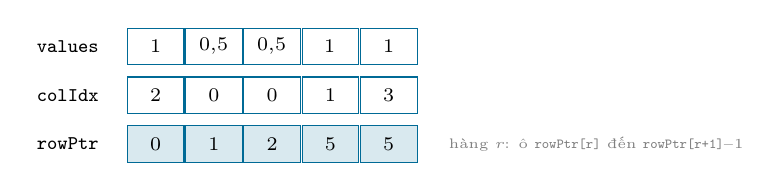
\begin{tikzpicture}[font=\scriptsize,
  cell/.style={draw=linkblue,minimum height=4.6mm,minimum width=7.2mm,inner sep=0.5pt}]
\node[anchor=east] at (-0.2,0) {\code{values}};
\foreach \i/\v in {0/1,1/0{,}5,2/0{,}5,3/1,4/1}
  \node[cell] at (\i*0.74+0.4,0) {$\v$};
\node[anchor=east] at (-0.2,-0.62) {\code{colIdx}};
\foreach \i/\v in {0/2,1/0,2/0,3/1,4/3}
  \node[cell] at (\i*0.74+0.4,-0.62) {\v};
\node[anchor=east] at (-0.2,-1.24) {\code{rowPtr}};
\foreach \i/\v in {0/0,1/1,2/2,3/5,4/5}
  \node[cell,fill=linkblue!15] at (\i*0.74+0.4,-1.24) {\v};
\node[anchor=west,font=\tiny,gray] at (4.0,-1.24) {hàng $r$: ô \code{rowPtr[r]} đến \code{rowPtr[r+1]}$-1$};
\end{tikzpicture}
\caption{Dạng CSR của ma trận liên kết cho đồ thị bốn trang A$\to$B, A$\to$C, B$\to$C, C$\to$A, D$\to$C. Hàng $j$ chứa các trang trỏ tới $j$ với trọng số $1/\text{out}$.}
\label{fig:csr}
\end{figure}

\srcref{lst:pagerank}

\subsection{Phần 4: Ghép tín hiệu}
\label{sec:boost}
Điểm cuối ghép ba tín hiệu: độ liên quan (TF-IDF hoặc BM25), PageRank và độ khớp tiêu đề. Bản đầu tiên cộng chúng với trọng số $0{,}6$ và $0{,}3$. Khi đo, em thấy cách cộng không hoạt động, vì các đại lượng khác thang nhau. Điểm TF-IDF trung bình là $0{,}178$ còn PageRank trung bình là $0{,}00035$. Sau khi nhân trọng số, PageRank chỉ đóng góp khoảng $0{,}1\%$ điểm cuối. Tăng trọng số của nó 16 lần cũng chỉ đổi MRR $0{,}004$.

Bản hiện tại nhân điểm cơ sở $s$ với một hệ số cho mỗi tín hiệu. Với PageRank, hệ số dùng giá trị đã chuẩn hóa về $[0,1]$ theo thang logarit:
\begin{equation}
s'=s\cdot\Big(1+\beta\,\frac{\ln\!\big(1+PR/PR_{\min}\big)}{\ln\!\big(1+PR_{\max}/PR_{\min}\big)}\Big).
\label{eq:prboost}
\end{equation}
Với tiêu đề, $\rho\in[0,1]$ là tỉ lệ âm tiết của truy vấn có mặt trong tiêu đề:
\begin{equation}
s''=s'\cdot(1+\gamma\,\rho).
\label{eq:titleboost}
\end{equation}
Phép nhân không phụ thuộc thang của $s$, nên đổi mô hình cơ sở từ TF-IDF (điểm cỡ $0{,}18$) sang BM25 (điểm cỡ 12) không đòi chỉnh lại $\beta$ và $\gamma$. Tài liệu có $s=0$ vẫn nhận điểm 0, tức uy tín không cứu được một tài liệu không liên quan.

Mỗi tín hiệu là một lớp bọc quanh \code{RelevanceScorer} (mẫu Decorator \cite{gamma1994design}). Nhờ vậy có thể bật tắt từng tín hiệu để đo đóng góp riêng của nó (Mục~\ref{chap:eval}).

\srcref{lst:prboost}

\subsection{Phần 5: Top-$K$ và bộ đệm}
\label{sec:topk}
\textbf{Top-$K$ bằng MinHeap.} Người dùng chỉ xem 10 kết quả đầu, nên sắp xếp cả tập ứng viên là thừa. Chương trình giữ một min-heap có đúng $K$ phần tử. Gốc heap là phần tử nhỏ nhất trong $K$ phần tử tốt nhất hiện có. Một ứng viên mới chỉ vào heap khi điểm của nó lớn hơn gốc, và khi đó gốc bị loại. Chi phí là $O(n\log K)$ thời gian và $O(K)$ bộ nhớ. Với 30.000 ứng viên và $K=10$, đó là khoảng 100.000 phép so sánh, còn sắp xếp toàn bộ cần khoảng 450.000.

$K$ phần tử đầu được gom lại rồi dựng heap một lần bằng \code{heapify} trong $O(K)$, thay vì chèn từng phần tử với $O(K\log K)$.

\srcref{lst:topk}

\textbf{LRU cache.} Các truy vấn phổ biến lặp lại nhiều. \code{LRUCache} giữ kết quả của 200 truy vấn gần nhất. Nó ghép một bảng băm với một danh sách liên kết đôi (Hình~\ref{fig:lru}). Bảng băm tìm nút trong $O(1)$. Danh sách giữ thứ tự sử dụng: nút vừa dùng được chuyển lên đầu, và khi đầy thì nút cuối bị loại. Hai nút giả ở hai đầu danh sách giúp thao tác thêm và xóa không phải xét trường hợp biên.

\begin{figure}[H]
\centering
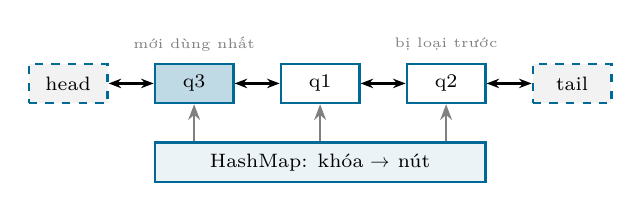
\begin{tikzpicture}[font=\scriptsize,
  nd/.style={draw=linkblue,thick,minimum height=5mm,minimum width=10mm,inner sep=1pt},
  sen/.style={nd,dashed,fill=gray!10}]
\node[sen] (h) at (0,0) {head};
\node[nd,fill=linkblue!25] (a) at (1.6,0) {q3};
\node[nd] (b) at (3.2,0) {q1};
\node[nd] (c) at (4.8,0) {q2};
\node[sen] (t) at (6.4,0) {tail};
\foreach \x/\y in {h/a,a/b,b/c,c/t}
  \draw[{Stealth[length=1.6mm]}-{Stealth[length=1.6mm]},thick] (\x)--(\y);
\node[draw=linkblue,thick,fill=linkblue!8,minimum width=42mm,minimum height=5mm] (map) at (3.2,-1.0) {HashMap: khóa $\to$ nút};
\draw[parr,gray] (map.north -| a)--(a);
\draw[parr,gray] (map.north -| b)--(b);
\draw[parr,gray] (map.north -| c)--(c);
\node[font=\tiny,gray] at (1.6,0.5) {mới dùng nhất};
\node[font=\tiny,gray] at (4.8,0.5) {bị loại trước};
\end{tikzpicture}
\caption{LRU cache: bảng băm cộng danh sách liên kết đôi có hai nút giả.}
\label{fig:lru}
\end{figure}

Hàm \code{get} lấy khóa ghi chứ không lấy khóa đọc, vì mỗi lần đọc đều đổi thứ tự của danh sách. Bộ đệm được tạo lại mỗi khi chỉ mục thay đổi, để kết quả cũ không còn được trả về. Crawler dùng cùng lớp này với sức chứa 1.000 để nhớ kết quả phân giải DNS.

\srcref{lst:lru}

%====================================================================
\section{P6: Gợi ý, dịch vụ và trình duyệt}
\label{chap:p6}
%====================================================================
Mục này trình bày phần người dùng nhìn thấy, gồm ba phần.
\begin{itemize}\itemsep0pt
\item Phần 1, gợi ý truy vấn: Trie theo ký tự.
\item Phần 2, cổng vào và xác thực.
\item Phần 3, trình duyệt mini.
\end{itemize}

\subsection{Phần 1: Gợi ý truy vấn}
\label{sec:suggest}
Khi người dùng gõ vào thanh địa chỉ, \code{/api/suggest} trả về các gợi ý bắt đầu bằng phần đã gõ. Dữ liệu nằm trong một Trie theo ký tự. Nút kết thúc một gợi ý lưu chuỗi hiển thị và tần suất. Tìm gợi ý gồm ba bước: đi theo tiền tố tới một nút, duyệt cả cây con của nút đó để gom các gợi ý, rồi lấy $K$ gợi ý có tần suất cao nhất bằng \code{MinHeap.topK}.

Mỗi gợi ý được chèn hai lần, một lần có dấu và một lần không dấu, cả hai cùng trỏ về chuỗi hiển thị có dấu. Người dùng gõ ``ha noi'' vẫn nhận được ``hà nội''. Vì chèn hai lần nên một tiền tố ngắn có thể chạm cả hai bản, và chương trình gộp các gợi ý trùng chuỗi hiển thị trước khi lấy top-$K$.

Nguồn gợi ý là từ ghép và cặp từ liền nhau trong tiêu đề các trang tiếng Việt, cộng với những truy vấn thật đã cho kết quả. Trie được xóa và dựng lại mỗi khi chỉ mục thay đổi.

\subsection{Phần 2: Cổng vào và xác thực}
Mọi request đi qua \code{api-gateway}. Cổng này định tuyến, kiểm tra JWT, giới hạn tốc độ bằng thuật toán token bucket và xử lý CORS. Có hai cách xác thực. Người dùng đăng nhập và nhận một access token JWT ký RS256 có hạn 15 phút, kèm một refresh token có hạn 30 ngày. Refresh token bị hủy ngay khi dùng và được thay bằng token mới. Công cụ dòng lệnh thì dùng khóa \code{X-API-Key} cố định khi gọi thẳng vào một dịch vụ.

Mật khẩu được băm bằng BCrypt với hệ số 12. Sau 5 lần đăng nhập sai, tài khoản bị khóa 15 phút. Ứng dụng từ chối khởi động nếu thiếu \code{ADMIN\_API\_KEY}, vì lệnh crawl của quản trị viên khiến máy chủ tải một URL do người gọi chọn.

Các bước của crawler nối với nhau qua một bus sự kiện. Mặc định bus chạy trong cùng tiến trình. Đổi một khóa cấu hình thì cùng các khối đó chạy qua Kafka trên nhiều tiến trình.

\subsection{Phần 3: Trình duyệt mini}
Giao diện là một ứng dụng Electron viết bằng React và TypeScript. Nó có tab, thanh địa chỉ kèm gợi ý, dấu trang, lịch sử, trang tải về, trang cài đặt và bảng quản trị. Hai cấu trúc dữ liệu được viết lại ở phía giao diện (Bảng~\ref{tab:frontend}).

\begin{table}[H]
\centering
\caption{Cấu trúc dữ liệu ở phía giao diện.}
\label{tab:frontend}
\footnotesize
\begin{tabular}{@{}p{2.2cm}p{5.4cm}@{}}
\toprule
Lớp & Dùng cho \\
\midrule
\code{Stack} & nút lùi và tiến: mỗi tab có một ngăn xếp lùi và một ngăn xếp tiến \\
\code{BookmarkTrie} & tìm dấu trang theo tiền tố khi gõ vào thanh địa chỉ \\
\bottomrule
\end{tabular}
\end{table}

Khi người dùng mở một trang mới, địa chỉ hiện tại được đẩy vào ngăn xếp lùi và ngăn xếp tiến bị xóa. Nút lùi lấy một địa chỉ khỏi ngăn xếp lùi và đẩy địa chỉ hiện tại sang ngăn xếp tiến. Nút tiến làm ngược lại.

Tiến trình chính của Electron từ chối điều hướng tới \code{file://} và \code{javascript:}. Quy tắc này được kiểm thử riêng vì nó là ranh giới bảo mật giữa nội dung web và máy của người dùng.

%====================================================================
\section{Đánh giá}
\label{chap:eval}
%====================================================================

\subsection{Độ phức tạp}
Bảng~\ref{tab:complexity} tổng hợp độ phức tạp của các thao tác chính.

\begin{table}[H]
\centering
\caption{Độ phức tạp của các cấu trúc dữ liệu và thuật toán.}
\label{tab:complexity}
\footnotesize
\begin{tabular}{@{}p{2.5cm}p{2.9cm}l@{}}
\toprule
Cấu trúc & Thao tác & Chi phí \\
\midrule
\code{MinHeap} & chèn, lấy nhỏ nhất & $O(\log n)$ \\
 & dựng từ $n$ phần tử & $O(n)$ \\
 & top-$K$ của $n$ & $O(n\log K)$ \\
\code{LRUCache} & \code{get}, \code{put} & $O(1)$ \\
\code{Trie} & chèn chuỗi dài $L$ & $O(L)$ \\
\code{SyllableTrie} & đi một cạnh & $O(1)$ trung bình \\
\code{BloomFilter} & thêm, kiểm tra & $O(k)$ \\
\code{SparseMatrix} & nhân với vector & $O(\text{nnz})$ \\
Tách từ & câu $n$ âm tiết & $O(n)$ \\
Giao posting list & hai con trỏ & $O(m+n)$ \\
 & \code{skipTo} & $O(\log d)$ \\
PageRank & một vòng lặp & $O(n+\text{nnz})$ \\
\bottomrule
\end{tabular}
\end{table}

\subsection{Chất lượng xếp hạng}
\label{sec:quality}
Đo chất lượng cần biết đáp án đúng của từng truy vấn. Em sinh truy vấn tự động theo kiểu \emph{known-item}: chọn một tài liệu, lấy ba term đặc trưng nhất của nó làm truy vấn, và coi chính tài liệu đó là đáp án duy nhất. Term đặc trưng là term có $tf\cdot idf$ cao, xuất hiện trong ít nhất 3 tài liệu và không quá 10\% corpus. Hạt ngẫu nhiên cố định ở 42, nên chạy lại cho đúng bộ truy vấn cũ.

Hai độ đo được dùng. MRR là trung bình của $1/r$, với $r$ là thứ hạng của đáp án. Success@1 là tỉ lệ truy vấn có đáp án đứng đầu. Bộ đo gọi đúng các lớp \code{QueryParser}, \code{CandidateResolver} và \code{ResultRanker} mà \code{/api/search} dùng. Bảng~\ref{tab:mrr} cho kết quả trên 200 truy vấn.

\begin{table}[H]
\centering
\caption{Chất lượng xếp hạng trên 200 truy vấn known-item.}
\label{tab:mrr}
\footnotesize
\begin{tabular}{@{}lrr@{}}
\toprule
Cấu hình & MRR & Success@1 \\
\midrule
TF-IDF & $0{,}8537$ & $78{,}0\%$ \\
BM25 & $0{,}8989$ & $85{,}0\%$ \\
TF-IDF + PageRank & $0{,}8625$ & \\
TF-IDF + tiêu đề & $0{,}9083$ & \\
\bottomrule
\end{tabular}
\end{table}

BM25 hơn TF-IDF khoảng $5{,}3\%$ MRR. Độ khớp tiêu đề thêm $0{,}0546$ vào MRR, gấp khoảng sáu lần mức $0{,}0088$ của PageRank. Điều này hợp với cách sinh truy vấn: term trong tiêu đề được ưu tiên khi chọn term đặc trưng, còn PageRank không biết gì về nội dung truy vấn.

Để biết một chênh lệch có phải do may rủi, bộ đo so hai cấu hình theo từng cặp truy vấn bằng hai phép kiểm định: t-test theo cặp và kiểm định hoán vị ngẫu nhiên với 100.000 lần hoán vị \cite{smucker2007}. Giá trị $1/r$ chỉ nhận các mức $1,\frac12,\frac13,\dots$ nên lệch xa phân phối chuẩn, và phép thứ hai không cần giả định đó. Một chênh lệch chỉ được coi là có ý nghĩa khi cả hai phép cho $p<0{,}05$.

Ngoài truy vấn sinh máy, dự án có 30 truy vấn tự nhiên viết tay để chấm theo nhãn do người gán (precision, recall, MAP, nDCG), và một bộ so sánh với chỉ mục GIN của PostgreSQL trên cùng corpus.

\subsection{Kiểm thử}
Backend có 661 bài kiểm thử, giao diện có 155. Bốn cổng chặn việc gộp mã (Bảng~\ref{tab:gates}). Cổng cuối dành riêng cho tìm kiếm: ba cổng đầu có thể đều qua trong khi kết quả trả cho người dùng đã kém đi.

\begin{table}[H]
\centering
\caption{Bốn cổng chất lượng trong CI.}
\label{tab:gates}
\footnotesize
\begin{tabular}{@{}p{2.6cm}p{5.0cm}@{}}
\toprule
Cổng & Bắt loại lỗi \\
\midrule
661 bài kiểm thử & sai logic của từng lớp \\
Độ phủ JaCoCo & mã mới không có kiểm thử (dòng $\ge68\%$, nhánh $\ge65\%$) \\
SpotBugs & lỗi mà không bài kiểm thử nào chạm tới \\
\code{RankingQualityTest} & chất lượng tìm kiếm giảm \\
\bottomrule
\end{tabular}
\end{table}

%====================================================================
\section{Hạn chế và hướng phát triển}
\label{chap:future}
%====================================================================
\subsection{Hạn chế}
\begin{itemize}\itemsep0pt
\item Chỉ mục nằm trọn trong bộ nhớ của một tiến trình. Corpus 39.780 tài liệu cho file chỉ mục $486{,}5$~MB, và lần khởi động đầu mất vài chục giây để dựng chỉ mục. Hệ thống chưa chia chỉ mục ra nhiều máy.
\item Bộ tách từ không hiểu ngữ cảnh. Nó chọn theo tổng trọng số từ điển, nên vẫn sai ở những câu mà cách tách đúng có tổng thấp hơn. Tên riêng không có trong từ điển bị tách thành từng âm tiết.
\item Truy vấn known-item dễ hơn truy vấn của người thật. MRR cao chỉ cho biết hệ thống tìm lại được một bài đã biết. Bộ 30 truy vấn có nhãn người gán còn nhỏ.
\item Bloom filter không xóa được phần tử, và 1\% dương tính giả nghĩa là một số trang không bao giờ được thăm.
\end{itemize}

\subsection{Hướng phát triển}
\begin{itemize}\itemsep0pt
\item Lập chỉ mục tăng dần. Hiện mỗi lần có corpus mới, chỉ mục được dựng lại từ đầu. Chia chỉ mục thành các đoạn bất biến rồi gộp dần sẽ cho phép thêm tài liệu mà không dừng tìm kiếm.
\item Giao posting list ngay trên dữ liệu nén. Hiện một khối phải được giải nén hết trước khi giao. Thêm bảng nhảy vào khối nén sẽ bỏ qua được các đoạn không cần đọc.
\item Sửa lỗi chính tả và truy vấn không dấu. Trie gợi ý đã xử lý trường hợp gõ không dấu, còn chỉ mục chính thì chưa.
\end{itemize}

%====================================================================
\section{Tuyên bố sử dụng AI}
\label{chap:ai}
%====================================================================
Theo quy định của môn học, sinh viên được dùng công cụ AI để học khái niệm, gỡ lỗi và cải thiện mã nguồn. Trong đồ án này, em đã dùng công cụ AI cho ba việc:
\begin{itemize}\itemsep0pt
\item Học khái niệm: giải thích chỉ mục đảo, VByte, BM25, PageRank, kiến trúc frontier của Mercator và các kỹ thuật liên quan.
\item Gỡ lỗi và cải thiện mã: tìm lỗi, gợi ý cách viết gọn và nhanh hơn cho chương trình.
\item Soạn tài liệu: hỗ trợ viết tài liệu kỹ thuật và bản thảo báo cáo này.
\end{itemize}
Em đã đọc, kiểm tra và chạy thử nội dung do AI gợi ý, và chịu trách nhiệm về toàn bộ mã nguồn và báo cáo này.

%====================================================================
\section{Kết luận}
\label{chap:end}
%====================================================================
CocCoc Plus tải trang, tách từ, lập chỉ mục, tìm và xếp hạng tài liệu tiếng Việt bằng các cấu trúc dữ liệu tự cài, và phục vụ kết quả cho một trình duyệt mini qua chín dịch vụ. Bảng~\ref{tab:src} liệt kê các file mã nguồn của từng phần.

\begin{table}[H]
\centering
\caption{Các file mã nguồn chính (trong \code{backend/java/libs/}).}
\label{tab:src}
\footnotesize
\begin{tabular}{@{}p{1.6cm}>{\raggedright\arraybackslash}p{6.1cm}@{}}
\toprule
Phần & File \\
\midrule
Cấu trúc dữ liệu & \mbox{\code{core-common/.../datastructure/}}: \mbox{\code{MinHeap}}, \mbox{\code{LRUCache}}, \mbox{\code{Trie}}, \mbox{\code{SyllableTrie}}, \mbox{\code{BloomFilter}}, \mbox{\code{SparseMatrix}} \\
P1 & \mbox{\code{core-crawler/.../frontier/UrlFrontier.java}}, \mbox{\code{BackQueues.java}}, \mbox{\code{WeightedRandomSelector.java}}, \mbox{\code{UrlSeenFilter.java}} \\
P2 & \mbox{\code{core-search/.../index/MaxWeightSegmenter.java}}, \mbox{\code{VietnameseWordDictionary.java}}, \mbox{\code{VietnameseTokenizer.java}} \\
P3 & \mbox{\code{index/InvertedIndex.java}}, \mbox{\code{VByteCodec.java}}, \mbox{\code{CompressedPostings.java}}, \mbox{\code{TermDictionary.java}} \\
P4 & \mbox{\code{query/QueryParser.java}}, \mbox{\code{PostingListMerger.java}}, \mbox{\code{CandidateResolver.java}}, \mbox{\code{query/ast/}} \\
P5 & \mbox{\code{ranking/TfIdfScorer.java}}, \mbox{\code{BM25Scorer.java}}, \mbox{\code{PageRankService.java}}, \mbox{\code{ResultRanker.java}}, \mbox{\code{ranking/decorator/}} \\
P6 & \mbox{\code{service/SuggestionService.java}}, \mbox{\code{services/api-gateway/}}, \mbox{\code{desktop-app/src/}} \\
Đánh giá & \mbox{\code{eval/EvaluationRunner.java}}, \mbox{\code{SignificanceTest.java}}, \mbox{\code{KnownItemQueryGenerator.java}} \\
\bottomrule
\end{tabular}
\end{table}

\begin{thebibliography}{99}\footnotesize\itemsep0pt\parskip0pt
\bibitem{manning2008ir} C.~D.~Manning, P.~Raghavan, H.~Sch{\"u}tze, Introduction to Information Retrieval, Cambridge University Press, 2008.
\bibitem{heydon1999mercator} A.~Heydon, M.~Najork, Mercator: a scalable, extensible web crawler, World Wide Web 2(4) (1999) 219--229.
\bibitem{bloom1970} B.~H.~Bloom, Space/time trade-offs in hash coding with allowable errors, Commun. ACM 13(7) (1970) 422--426.
\bibitem{coccoctokenizer} Cốc Cốc, coccoc-tokenizer: a Vietnamese tokenizer, \url{https://github.com/coccoc/coccoc-tokenizer}.
\bibitem{salton1988} G.~Salton, C.~Buckley, Term-weighting approaches in automatic text retrieval, Inf. Process. Manag. 24(5) (1988) 513--523.
\bibitem{robertson2009bm25} S.~Robertson, H.~Zaragoza, The probabilistic relevance framework: BM25 and beyond, Found. Trends Inf. Retr. 3(4) (2009) 333--389.
\bibitem{brin1998} S.~Brin, L.~Page, The anatomy of a large-scale hypertextual web search engine, Comput. Netw. ISDN Syst. 30(1--7) (1998) 107--117.
\bibitem{smucker2007} M.~D.~Smucker, J.~Allan, B.~Carterette, A comparison of statistical significance tests for information retrieval evaluation, in: CIKM, 2007, pp.~623--632.
\bibitem{gamma1994design} E.~Gamma, R.~Helm, R.~Johnson, J.~Vlissides, Design Patterns: Elements of Reusable Object-Oriented Software, Addison-Wesley, 1994.
\end{thebibliography}


%====================================================================
% PHỤ LỤC: toàn bộ đoạn mã, một cột
%====================================================================
\clearpage
\onecolumn
\appendix
\lstset{language=Java,basicstyle=\ttfamily\fontsize{7.2}{8.6}\selectfont,numbers=left,numberstyle=\tiny\color{gray},
  numbersep=6pt,xleftmargin=16pt,framexleftmargin=14pt,frame=single,rulecolor=\color{gray!60},
  backgroundcolor=\color{gray!5},framerule=0.5pt,aboveskip=6pt,belowskip=10pt,
  breaklines=true,breakindent=0pt,captionpos=t}
\captionsetup[lstlisting]{skip=4pt,font={small,bf},labelfont=bf}
\section{Mã nguồn các đoạn code}
\label{app:code}
Mọi đoạn code đều được trích từ chương trình, đã lược phần chú thích Javadoc. Phần nội dung chính dẫn tới từng đoạn bằng số thứ tự.

\subsection{P1: Thu thập trang web}
\begin{minipage}{\linewidth}
\begin{lstlisting}[caption={\code{frontier/WeightedRandomSelector.java}, \code{select}: chọn hàng đợi tầng trước theo trọng số $2^{L-1-i}$},label={lst:selector}]
@Override
public int select(int[] queueSizes) {
    int levels = queueSizes.length;
    if (levels > MAX_LEVELS) {
        throw new IllegalArgumentException(
                "Chỉ hỗ trợ tối đa " + MAX_LEVELS + " mức, nhận được: " + levels);
    }
    long totalWeight = 0;
    for (int i = 0; i < levels; i++) {
        if (queueSizes[i] > 0) {
            totalWeight += weightOf(i, levels);
        }
    }
    if (totalWeight == 0) {
        return -1; // mọi hàng đợi đều rỗng
    }
    long pick = Math.floorMod(random.nextLong(), totalWeight);
    for (int i = 0; i < levels; i++) {
        if (queueSizes[i] == 0) {
            continue;
        }
        pick -= weightOf(i, levels);
        if (pick < 0) {
            return i;
        }
    }
    throw new IllegalStateException("Không chọn được hàng đợi dù tổng trọng số > 0");
}

private static long weightOf(int level, int levels) {
    return 1L << (levels - 1 - level);
}
\end{lstlisting}
\end{minipage}
\par\vspace{4pt}

\begin{minipage}{\linewidth}
\begin{lstlisting}[caption={\code{frontier/BackQueues.java}, \code{poll}: lấy URL của host tới giờ sớm nhất},label={lst:backpoll}]
public CrawlTask poll(long now) {
    if (ready.isEmpty()) {
        return null;
    }
    int slot = ready.peek();
    if (availableAt[slot] > now) {
        return null; // phần tử nhỏ nhất chưa tới giờ => không có phần tử nào tới giờ
    }
    ready.extractMin();
    inReady[slot] = false; // từ đây tới lúc chèn lại, availableAt[slot] mới được phép đổi
    CrawlTask task = queues.get(slot).pollFirst();
    pending--;
    availableAt[slot] = now + politenessDelayMs;
    if (queues.get(slot).isEmpty()) {
        markEmpty(slot);
    } else {
        ready.insert(slot);
        inReady[slot] = true;
    }
    return task;
}
\end{lstlisting}
\end{minipage}
\par\vspace{4pt}

\begin{minipage}{\linewidth}
\begin{lstlisting}[caption={\code{datastructure/BloomFilter.java}: tính $m$, $k$ và băm kép},label={lst:bloom}]
public BloomFilter(int expectedItems, double falsePositiveRate) {
    if (expectedItems <= 0) {
        throw new IllegalArgumentException("expectedItems phải > 0");
    }
    if (falsePositiveRate <= 0 || falsePositiveRate >= 1) {
        throw new IllegalArgumentException("falsePositiveRate phải trong khoảng (0, 1)");
    }
    double ln2 = Math.log(2);
    int m = (int) Math.ceil(-expectedItems * Math.log(falsePositiveRate) / (ln2 * ln2));
    m = Math.max(m, 64);
    int k = (int) Math.round((double) m / expectedItems * ln2);
    this.numBits = m;
    this.numHashes = Math.max(k, 1);
    this.bits = new long[(m + 63) / 64];
}

public boolean mightContain(String item) {
    long h1 = hash1(item);
    long h2 = hash2(item);
    for (int i = 0; i < numHashes; i++) {
        int idx = indexFor(h1, h2, i);
        if (!getBit(idx)) {
            return false;
        }
    }
    return true;
}

private int indexFor(long h1, long h2, int i) {
    long combined = h1 + (long) i * h2;
    return (int) Math.floorMod(combined, (long) numBits);
}

private static long hash1(String s) {
    byte[] data = s.getBytes(StandardCharsets.UTF_8);
    long hash = 0xcbf29ce484222325L; // FNV offset basis
    for (byte b : data) {
        hash ^= (b & 0xffL);
        hash *= 0x100000001b3L; // FNV prime
    }
    return hash;
}
\end{lstlisting}
\end{minipage}
\par\vspace{4pt}

\subsection{P2: Tách từ tiếng Việt}
\begin{minipage}{\linewidth}
\begin{lstlisting}[caption={\code{index/MaxWeightSegmenter.java}, \code{segment}, \code{relax}, \code{traceBack}: quy hoạch động tách từ},label={lst:segment}]
public int[] segment(String[] syllables) {
    int n = syllables.length;
    if (n == 0) {
        return new int[]{0};
    }
    double[] best = new double[n + 1];
    int[] trace = new int[n + 1];
    java.util.Arrays.fill(best, Double.NEGATIVE_INFINITY);
    best[0] = 0.0;
    trace[0] = -1;
    for (int i = 0; i < n; i++) {
        if (best[i] == Double.NEGATIVE_INFINITY) {
            continue;
        }
        relax(best, trace, i + 1, best[i] + unknownSyllableWeight, i);
        int node = trie.root();
        int maxEnd = Math.min(n, i + VietnameseWordDictionary.MAX_SYLLABLES);
        for (int j = i; j < maxEnd; j++) {
            node = trie.child(node, trie.idOf(syllables[j]));
            if (node == SyllableTrie.NONE) {
                break;
            }
            if (trie.isWord(node)) {
                relax(best, trace, j + 1, best[i] + trie.weightAt(node), i);
            }
        }
    }
    return traceBack(trace, n);
}

private static void relax(double[] best, int[] trace, int to, double score, int from) {
    if (score > best[to]) {
        best[to] = score;
        trace[to] = from;
    }
}

private static int[] traceBack(int[] trace, int n) {
    int count = 0;
    for (int i = n; i > 0; i = trace[i]) {
        count++;
    }
    int[] boundaries = new int[count + 1];
    boundaries[count] = n;
    int k = count;
    for (int i = n; i > 0; i = trace[i]) {
        boundaries[--k] = trace[i];
    }
    return boundaries;
}
\end{lstlisting}
\end{minipage}
\par\vspace{4pt}

\subsection{P3: Chỉ mục đảo và nén}
\begin{minipage}{\linewidth}
\begin{lstlisting}[caption={\code{index/VByteCodec.java}, \code{encodeSorted}, \code{writeVInt}, \code{readVInt}: delta và VByte},label={lst:vbyte}]
public static byte[] encodeSorted(int[] sorted) {
    if (sorted == null || sorted.length == 0) {
        return new byte[0];
    }
    ByteArrayOutputStream out = new ByteArrayOutputStream(sorted.length);
    int previous = 0;
    for (int i = 0; i < sorted.length; i++) {
        int value = sorted[i];
        if (value < 0) {
            throw new IllegalArgumentException("VByte chi ma hoa so khong am, gap: " + value);
        }
        if (i > 0 && value < previous) {
            throw new IllegalArgumentException(
                    "Danh sach phai tang dan; vi tri " + i + " co " + value + " < " + previous);
        }
        writeVInt(out, value - previous); // delta
        previous = value;
    }
    return out.toByteArray();
}

private static void writeVInt(ByteArrayOutputStream out, int value) {
    while ((value & ~0x7F) != 0) {          // con bit ngoai 7 bit thap
        out.write((value & 0x7F) | 0x80);   // ghi 7 bit + bat co "con nua"
        value >>>= 7;
    }
    out.write(value & 0x7F);                // byte cuoi: bit cao = 0
}

private static long readVInt(byte[] data, int position) {
    int value = 0;
    int shift = 0;
    while (true) {
        if (position >= data.length) {
            throw new IllegalArgumentException("Du lieu VByte bi cat cut tai vi tri " + position);
        }
        int b = data[position++] & 0xFF;
        value |= (b & 0x7F) << shift;
        if ((b & 0x80) == 0) {
            break; // bit cao = 0 -> byte cuoi
        }
        shift += 7;
        if (shift > 28) {
            throw new IllegalArgumentException("So VByte vuot qua pham vi int 32-bit");
        }
    }
    return ((long) position << 32) | (value & 0xFFFFFFFFL);
}
\end{lstlisting}
\end{minipage}
\par\vspace{4pt}

\subsection{P4: Xử lý truy vấn}
\begin{minipage}{\linewidth}
\begin{lstlisting}[caption={\code{index/ArrayPostingCursor.java}, \code{skipTo}: nhảy theo cấp số nhân rồi tìm nhị phân},label={lst:skipto}]
@Override
public boolean skipTo(int targetDocId) {
    int n = postings.size();
    if (index >= n) {
        return false;
    }
    if (postings.get(index).docId() >= targetDocId) {
        return true; // da o dung cho hoac vuot qua roi
    }

    // --- Pha 1: nhay theo cap so nhan ---
    int step = 1;
    int low = index;
    int high = index + step;
    while (high < n && postings.get(high).docId() < targetDocId) {
        low = high;
        step <<= 1;                    // 1, 2, 4, 8, ...
        high = index + step;
    }
    if (high >= n) {
        high = n - 1;
    }

    // --- Pha 2: binary search trong doan (low, high] ---
    int lo = low;
    int hi = high;
    while (lo < hi) {
        int mid = (lo + hi) >>> 1;     // >>> chong tran
        if (postings.get(mid).docId() < targetDocId) {
            lo = mid + 1;
        } else {
            hi = mid;
        }
    }

    index = postings.get(lo).docId() >= targetDocId ? lo : n;
    return index < n;
}
\end{lstlisting}
\end{minipage}
\par\vspace{4pt}

\begin{minipage}{\linewidth}
\begin{lstlisting}[caption={\code{query/PostingListMerger.java}, \code{intersectCursors}, \code{intersectAll}: giao posting list, danh sách ngắn trước},label={lst:intersect}]
public static List<Integer> intersectCursors(PostingCursor a, PostingCursor b) {
    List<Integer> result = new ArrayList<>();
    while (a.docId() != PostingCursor.NO_MORE && b.docId() != PostingCursor.NO_MORE) {
        int docA = a.docId();
        int docB = b.docId();
        if (docA == docB) {
            result.add(docA);
            a.next();
            b.next();
        } else if (docA < docB) {
            a.skipTo(docB); // nhảy cóc thay vì next() từng bước
        } else {
            b.skipTo(docA);
        }
    }
    return result;
}

public static List<Integer> intersectAll(List<List<Posting>> postingLists) {
    if (postingLists.isEmpty()) {
        return new ArrayList<>();
    }
    List<List<Posting>> sorted = new ArrayList<>(postingLists);
    sorted.sort(Comparator.comparingInt(List::size)); // shortest-first
    if (sorted.size() == 1) {
        return docIdsOf(sorted.get(0));
    }
    List<Integer> result = intersectCursors(
            PostingCursor.of(sorted.get(0)), PostingCursor.of(sorted.get(1)));
    for (int i = 2; i < sorted.size() && !result.isEmpty(); i++) {
        result = intersectCursorWithList(PostingCursor.of(sorted.get(i)), result);
    }
    return result;
}
\end{lstlisting}
\end{minipage}
\par\vspace{4pt}

\subsection{P5: Xếp hạng}
\begin{minipage}{\linewidth}
\begin{lstlisting}[caption={\code{ranking/BM25Scorer.java}, \code{idf}, \code{prepare}: tính idf một lần, chấm từng tài liệu},label={lst:bm25}]
public static double idf(int totalDocs, int documentFrequency) {
    if (documentFrequency <= 0 || totalDocs <= 0) {
        return 0.0;
    }
    return Math.log(1 + ((double) totalDocs - documentFrequency + 0.5) / (documentFrequency + 0.5));
}

@Override
public DocumentScorer prepare(Map<String, Integer> queryTermFrequency, SearchIndex index) {
    int totalDocs = index.getTotalDocs();
    double avgDocLength = index.getAverageDocLength();
    if (totalDocs == 0 || avgDocLength <= 0) {
        return docId -> 0.0;
    }
    int size = queryTermFrequency.size();
    String[] terms = new String[size];
    double[] idfValues = new double[size];
    int kept = 0;
    for (String term : queryTermFrequency.keySet()) {
        int df = index.getDocumentFrequency(term);
        if (df == 0) {
            continue;
        }
        terms[kept] = term;
        idfValues[kept] = idf(totalDocs, df);
        kept++;
    }
    final int count = kept;
    if (count == 0) {
        return docId -> 0.0;
    }
    return docId -> {
        double lengthNorm = k1 * (1 - b + b * (index.getDocLength(docId) / avgDocLength));
        double total = 0.0;
        for (int i = 0; i < count; i++) {
            int termFrequency = index.getTermFrequency(terms[i], docId);
            if (termFrequency == 0) {
                continue;
            }
            total += idfValues[i] * (termFrequency * (k1 + 1)) / (termFrequency + lengthNorm);
        }
        return total;
    };
}
\end{lstlisting}
\end{minipage}
\par\vspace{4pt}

\begin{minipage}{\linewidth}
\begin{lstlisting}[caption={\code{ranking/PageRankService.java}, \code{computePageRank}: dựng ma trận thưa và vòng lặp lũy thừa (trích)},label={lst:pagerank}]
SparseMatrix incoming = new SparseMatrix(n, n);
boolean[] dangling = new boolean[n];
for (int idx = 0; idx < n; idx++) {
    if (outDegree[idx] == 0) {
        dangling[idx] = true;
        continue;
    }
    double weight = 1.0 / outDegree[idx];
    WebDocument doc = documents.get(docIds.get(idx));
    for (String outlink : doc.getOutlinks()) {
        Integer targetIdx = urlToIndex.get(outlink);
        if (targetIdx != null && targetIdx != idx) {
            incoming.set(targetIdx, idx, weight);
        }
    }
}
incoming.freeze();

double[] pr = new double[n];
for (int i = 0; i < n; i++) {
    pr[i] = 1.0 / n;
}
int iteration = 0;
double diff;
double teleport = (1 - DAMPING) / n;
do {
    double danglingSum = 0.0;
    for (int i = 0; i < n; i++) {
        if (dangling[i]) {
            danglingSum += pr[i];
        }
    }
    double danglingContribution = DAMPING * danglingSum / n;
    double[] linkContribution = incoming.multiply(pr);
    double[] newPr = new double[n];
    diff = 0.0;
    for (int j = 0; j < n; j++) {
        newPr[j] = teleport + DAMPING * linkContribution[j] + danglingContribution;
        diff += Math.abs(newPr[j] - pr[j]);
    }
    pr = newPr;
    iteration++;
} while (diff >= EPSILON && iteration < MAX_ITERATIONS);
\end{lstlisting}
\end{minipage}
\par\vspace{4pt}

\begin{minipage}{\linewidth}
\begin{lstlisting}[caption={\code{ranking/decorator/PageRankBoostScorer.java}, \code{prepare}: nhân điểm cơ sở với hệ số PageRank},label={lst:prboost}]
@Override
public DocumentScorer prepare(Map<String, Integer> queryTermFrequency, SearchIndex index) {
    DocumentScorer base = inner.prepare(queryTermFrequency, index);
    if (weight == 0.0) {
        return base; // tin hieu bi tat: khong boc them lop nao
    }
    return docId -> {
        double baseScore = base.score(docId);
        if (baseScore == 0.0) {
            return baseScore; // thoat som: uy tin khong cuu duoc tai lieu khong lien quan
        }
        double pageRank = pageRankScores.getOrDefault(docId, minPageRank);
        double normalized = Math.log1p(pageRank / minPageRank) / logRange; // thuoc [0, 1]
        return baseScore * (1 + weight * normalized);
    };
}
\end{lstlisting}
\end{minipage}
\par\vspace{4pt}

\begin{minipage}{\linewidth}
\begin{lstlisting}[caption={\code{datastructure/MinHeap.java}, \code{topK}, \code{siftDown}: lấy $K$ phần tử lớn nhất},label={lst:topk}]
public static <T> List<T> topK(Collection<T> items, int k, Comparator<T> cmp) {
    if (k <= 0 || items == null || items.isEmpty()) {
        return new ArrayList<>();
    }
    List<T> seed = new ArrayList<>(Math.min(k, items.size()));
    MinHeap<T> heap = null;
    for (T item : items) {
        if (heap == null) {
            seed.add(item);
            if (seed.size() == k) {
                heap = new MinHeap<>(seed, cmp);
            }
            continue;
        }
        if (cmp.compare(item, heap.peek()) > 0) {
            heap.extractMin();
            heap.insert(item);
        }
    }
    if (heap == null) {
        heap = new MinHeap<>(seed, cmp); // items.size() < k
    }
    List<T> result = new ArrayList<>(heap.size());
    while (!heap.isEmpty()) {
        result.add(heap.extractMin()); // ra theo thứ tự TĂNG dần
    }
    java.util.Collections.reverse(result); // đảo lại thành GIẢM dần
    return result;
}

private void siftDown(int index) {
    int n = heap.size();
    int half = n >>> 1;
    T item = heap.get(index);
    while (index < half) {
        int child = 2 * index + 1;
        int right = child + 1;
        T childItem = heap.get(child);
        if (right < n) {
            T rightItem = heap.get(right);
            if (comparator.compare(rightItem, childItem) < 0) {
                child = right; // phải chọn con NHỎ hơn, nếu không vi phạm min-heap
                childItem = rightItem;
            }
        }
        if (comparator.compare(childItem, item) >= 0) {
            break;
        }
        heap.set(index, childItem);
        index = child;
    }
    heap.set(index, item);
}
\end{lstlisting}
\end{minipage}
\par\vspace{4pt}

\begin{minipage}{\linewidth}
\begin{lstlisting}[caption={\code{datastructure/LRUCache.java}, \code{get}, \code{put} và các thao tác trên danh sách},label={lst:lru}]
public V get(K key) {
    lock.writeLock().lock();
    try {
        Node<K, V> node = map.get(key);
        if (node == null) {
            return null;
        }
        moveToFront(node);
        return node.value;
    } finally {
        lock.writeLock().unlock();
    }
}

public void put(K key, V value) {
    lock.writeLock().lock();
    try {
        Node<K, V> existing = map.get(key);
        if (existing != null) {
            existing.value = value;
            moveToFront(existing);
            return;
        }
        Node<K, V> node = new Node<>(key, value);
        map.put(key, node);
        addToFront(node);
        if (map.size() > capacity) {
            Node<K, V> lru = tail.prev;
            removeNode(lru);
            map.remove(lru.key);
        }
    } finally {
        lock.writeLock().unlock();
    }
}

private void addToFront(Node<K, V> node) {
    node.prev = head;
    node.next = head.next;
    head.next.prev = node;
    head.next = node;
}

private void removeNode(Node<K, V> node) {
    node.prev.next = node.next;
    node.next.prev = node.prev;
}

private void moveToFront(Node<K, V> node) {
    removeNode(node);
    addToFront(node);
}
\end{lstlisting}
\end{minipage}

\end{document}
